% !TEX program = xelatex
\documentclass[aspectratio=169,9pt,handout]{beamer}
\usetheme{Compostela}
\usepackage{amsmath,bm}

%\usepackage{pgfpages}
%\setbeameroption{show notes on second screen}

\usepackage{pdfcomment}
%\newcommand{\pdfnote}[1]{\marginnote{\pdfcomment[icon=note]{#1}}}
\newcommand{\pdfnote}[1]{}


%%%%%%%%%%%%%%%%%%%%%%%%%%%%%%%%%%%%%%%%%%%%%%%%%%%%%%%%%%%%%%%%%%%%%%%%%%%%%%%%
%%%%%%%%%%%%%%%%%%%%%%%%%%%% Talk Configuration %%%%%%%%%%%%%%%%%%%%%%%%%%%%%%%%

\newcommand{\TalkPlace}{A \& S week}
\newcommand{\TalkAuthor}{
\href{mailto:marcos.romero.lamas@cern.ch}{Marcos Romero Lamas}\\
for the $\phi_s$ group
}
\newcommand{\TalkAuthorShort}{Marcos Romero}
\newcommand{\TalkTitle}{\Huge Acceptances and\\ resolutions in\\ $B_s^0 \rightarrow J/\psi \phi$}
\newcommand{\TalkTitleShort}{Acceptances and resolutions in $B_s^0 \rightarrow J/\psi \phi$}
\newcommand{\TalkInstitute}{}
\newcommand{\TalkDate}{October 27th}
\newcommand{\TalkDateNumber}{2020/10/27}

%%%%%%%%%%%%%%%%%%%%%%%%%%%%%%%%%%%%%%%%%%%%%%%%%%%%%%%%%%%%%%%%%%%%%%%%%%%%%%%%

\usepackage{adjustbox,multicol}

\usepackage{tikz,shapepar,booktabs}
\newcommand{\myparshape}{
{20}
{0}b{20}\\ 
{0}t{7.5}{20}\\ % corta arriba
{20}t{0}{30}\\  % corta abaixo
{20}e{10}
}

\usepackage{lipsum}

\usepackage{array}
\newcommand{\TupleVersion}{v0r5}
\newcommand{\FIGS}{/home3/marcos.romero/phis-scq/output/figures}
\newcommand{\PARS}{/home3/marcos.romero/phis-scq/output/tables}

\newenvironment{variableblock}[3]{%
  \setbeamercolor{block body}{#2}
  \setbeamercolor{block title}{#3}
  \begin{block}{#1}}{\end{block}}

%%%%%%%%%%%%%%%%%%%%%%%%%%%%%%%%%%%%%%%%%%%%%%%%%%%%%%%%%%%%%%%%%%%%%%%%%%%%%%%%
\begin{document} %%%%%%%%%%%%%%%%%%%%%%%%%%%%%%%%%%%%%%%%%%%%%%%%%%%%%%%%%%%%%%%
%%%%%%%%%%%%%%%%%%%%%%%%%%%%%%%%%%%%%%%%%%%%%%%%%%%%%%%%%%%%%%%%%%%%%%%%%%%%%%%%



%%%%%%%%%%%%%%%%%%%%%%%%%%%%%%%%%%%%%%%%%%%%%%%%%%%%%%%%%%%%%%%%%%%%%%%%%%%%%%%%
%%%%%%%%%%%%%%%%%%%%%%%%%%%%% TITLE PAGE & CONTENTS %%%%%%%%%%%%%%%%%%%%%%%%%%%%
%%%%%%%%%%%%%%%%%%%%%%%%%%%%%%%%%%%%%%%%%%%%%%%%%%%%%%%%%%%%%%%%%%%%%%%%%%%%%%%%

\begin{frame}[plain,overlaytitlepage=0.9,backgroundpicture=gpx/aiandes.pdf]
  \begin{minipage}[b][\textheight][b]{5cm}
    \includegraphics[height=0.5cm]{logos/igfae_bw}\hspace{1mm}
    \includegraphics[height=0.5cm]{logos/usc_bw}\hspace{1mm}
    \includegraphics[height=0.5cm]{logos/xunta_bw}\hspace{1mm}\\[2mm]
    \includegraphics[height=0.5cm]{logos/maeztu_bw}\hspace{1mm}
    \includegraphics[height=0.5cm]{logos/lhcb_bw}\\[-1mm]
  \end{minipage}
\end{frame}

\begin{frame}[plain,backgroundpicture=gpx/aiandes.pdf,overlaytoc=0.9]
  \addtocounter{framenumber}{-1}
  \hspace*{8cm}\begin{minipage}{8cm}
    \tableofcontents
  \end{minipage}
  \pdfnote{The talk consists in a brief overview of the Bs2JpsiPhi channel and the selection.}
  \pdfnote{Then I will talk about the meat of this talk: decay-time resolution and acceptance}
  \pdfnote{Then I will talk a bit of angular accepntace and finally a sneak peek of Preliminary fit resutls of the full run2 analysis.}
\end{frame}

%%%%%%%%%%%%%%%%%%%%%%%%%%%%%%%%%%%%%%%%%%%%%%%%%%%%%%%%%%%%%%%%%%%%%%%%%%%%%%%%






%%%%%%%%%%%%%%%%%%%%%%%%%%%%%%%%%%%%%%%%%%%%%%%%%%%%%%%%%%%%%%%%%%%%%%%%%%%%%%%%
%%%%%%%%%%%%%%%%%%%%%%%%%%%%%%%%%%%%%%%%%%%%%%%%%%%%%%%%%%%%%%%%%%%%%%%%%%%%%%%%
\section{Overview}
%%%%%%%%%%%%%%%%%%%%%%%%%%%%%%%%%%%%%%%%%%%%%%%%%%%%%%%%%%%%%%%%%%%%%%%%%%%%%%%%
%%%%%%%%%%%%%%%%%%%%%%%%%%%%%%%%%%%%%%%%%%%%%%%%%%%%%%%%%%%%%%%%%%%%%%%%%%%%%%%%



%\section{Selection}

\begin{frame}[default] % -------------------------------------------------------
\frametitle{nosubsection}

\begin{columns}[T]

  \begin{column}{0.4\paperwidth}

    \begin{description}[Go0al]
      \item[Goal] Measure the phase difference between amplitudes with and without oscillation in $B^0_s \rightarrow c\bar{c}s$ decays: $\phi_s$. {\small
          $$ \phi_s^{\text{SM}} \approx -2\arg\left(-\frac{V_{ts}V_{tb}^{*}}{V_{cs}V_{cb}^{*}}\right)\equiv-2\beta_{s}. $$}
      %\vspace*{-7mm}
      \begin{itemize}
        \item $\Gamma_s - \Gamma_d$ measurement, testing HQE.
        \item $\Delta \Gamma_s \equiv \frac{\Gamma_L - \Gamma_H}{2}$.
        \item $\Delta m_s \equiv m_H - m_L$.
      \end{itemize} 
      \item[Why] Sensitive probe of NP in $B_s^0$ mixing.
      \item[How] Current WA is dominated by LHC$b$ and main precision comes from $B_s^0 \rightarrow J/\psi K^+ K^- $ in $\phi$ region.
      \begin{itemize}
        \item Clean experimental signature.
        \item Relatively high BR, $\mathcal{O}(10^{-3})$.
        \item Small penguin pollution.
      \end{itemize}
    \end{description}

  \end{column}
  
  \begin{column}{0.55\textwidth}
    
    \begin{columns}%[T]

      \begin{column}{0.475\textwidth}
        \begin{variableblock}{$\phi_s$ CKMfitter\\ SM prediction}{bg=gray!20}{bg=gray}
         \centering  $\phi_s = -0.03696_{-0.00072}^{+0.00084}$ rad
        \end{variableblock}
        \begin{variableblock}{SM prediction}{bg=gray!20}{bg=gray}
         \centering  $\Delta \Gamma =  0.088 \pm 0.020\, \mathsf{ps}^{-1}$
         \centering  $\Gamma_s {}^{\dagger} = 0.6587 \pm 0.0024 \, \mathsf{ps}^{-1}$ 
        \end{variableblock}

        \begin{center}
          \href{http://ckmfitter.in2p3.fr}{\beamerbutton{CKMfitter}}
          \href{https://arxiv.org/pdf/1511.09466.pdf}{\beamerbutton{Artuso et al}} \\
          \href{https://cds.cern.ch/record/2668482/files/ATLAS-CONF-2019-009.pdf}{\beamerbutton{ATLAS}}
          \href{http://cds.cern.ch/record/2722794/files/BPH-20-001-arXiv.pdf}{\beamerbutton{CMS}}
          \href{https://arxiv.org/abs/1906.08356}{\beamerbutton{LHC$b$}}
        \end{center}

        \scriptsize
        \rule{3cm}{0.1mm} \\
        \dagger: \\ Theory predicts $\frac{\Gamma_s}{\Gamma_d} = 1.0006\pm0.0025$. $\Gamma_s$ is computed using the current WA $\Gamma_d = 1.519\pm 0.004$

      \end{column}



      \begin{column}{0.475\textwidth}

        \small 
        \begin{variableblock}{ATLAS}{bg=scqblue!20}{bg=scqblue}
          \centering $\phi_s = -0.076 \pm 0.034 \pm 0.019$ rad
          \centering $\Delta \Gamma = 0.068 \pm 0.004 \pm 0.003 \, \mathsf{ps}^{-1}$ 
          \centering $\Gamma_s = 0.669 \pm 0.001 \pm 0.001 \, \mathsf{ps}^{-1}$ 
        \end{variableblock}

        \small 
        \begin{variableblock}{CMS}{bg=scqred!20}{bg=scqred}
          \centering $\phi_s = -0.021 \pm 0.045$ rad 
          \centering $\Delta \Gamma = 0.1073 \pm 0.0097 \, \mathsf{ps}^{-1}$  
          \centering $\Gamma_s\!=\!0.6531\!\pm\!0.0042\!\pm\!0.0024\, \mathsf{ps}^{-1}$  
        \end{variableblock}
        
        \normalsize
        \begin{variableblock}{LHC$b$}{bg=scqgreen!20}{bg=scqgreen}
          \centering $\phi_s = -0.041 \pm 0.025$ rad 
          \centering $\Delta \Gamma = 0.0813 \pm 0.0048 \, \mathsf{ps}^{-1}$  
          \centering $\Gamma_s = 0.6563 \pm 0.0021 \, \mathsf{ps}^{-1}$  
        \end{variableblock}

      \end{column}

    \end{columns}



  \end{column}
  
\end{columns}

\pdfnote{Our goal is to meassure the oscillation phase in B2ccs oscillations, the so called phis which is well predicted to be -2 beta s in the SM}
\pdfnote{Besides that, we also measure Gs via Gs minus Gd, DGs and DMs}
\pdfnote{Bs2JpsiPhi is the golden channel to measure phis. Cause it has a clean experimenal signature, a relative high branching fraction and it has a theoreticaly small penguin pollution}

\end{frame} % ------------------------------------------------------------------


\subsection*{Ingredients}
\begin{frame}[default] % -------------------------------------------------------
\frametitle{noframetitle}

\begin{columns}%[T]
  \begin{column}{0.45\textwidth}
    \begin{variableblock}{Time-dependent asymmetry in the SM}{bg=scqblue!20}{bg=scqblue}
      \centering $\mathcal{A}_{\text{CP}} = \frac{\Gamma[\overline{B}{}_s^0 \rightarrow f] - \Gamma[{B}{}_s^0 \rightarrow f]}{\Gamma[\overline{B}{}_s^0 \rightarrow f] + \Gamma[{B}{}_s^0 \rightarrow f]} \approx \eta \sin \phi_s \sin \Delta m_s t $
    \end{variableblock}
    \tiny \hspace*{-5mm}
    \[p.d.f. = \frac{\displaystyle
      \sum_{u,v={S,0,\parallel,\perp}} \!\!\!  
        C_{u,v} 
        \,\,\, 
        A_{u} \overline{A}_{v}
        \,\,\, 
        f_{u,v} [\Omega]
        \,\,\,  \left\{  
        h_{u,v}^{B_s^0}[t] +  
        h_{u,v}^{\overline{B}_0^s}[t]  \right\}
      }{\displaystyle \int_{0.3 \, \text{ps}}^{15 \, \text{ps}}dt \int_{\Omega} d\Omega
      \sum_{u,v={S,0,\parallel,\perp}} \!\!\!  
        \,\,\, 
        A_{u} \overline{A}_{v}
        \,\,\, 
        f_{u,v} [\Omega]
        \,\,\,  \left\{  
        h_{u,v}^{B_s^0}[t] +  
        h_{u,v}^{\overline{B}_0^s}[t]  \right\} 
      }\]
    
      \begin{center}
        \includegraphics[width=0.6\textwidth]{gpx/HelicityPlanes}
      \end{center}
  \end{column}

  \begin{column}{0.45\textwidth}
    \begin{variableblock}{We experimentally measure }{bg=scqorange!20}{bg=scqorange}
      \centering $\mathcal{A}_{\text{CP}} \approx  (1-2\omega) e^{-\frac{1}{2} {\Delta m_s}^2 {\sigma_t}^2 } \eta \sin \phi_s \sin \Delta m_s t $
    \end{variableblock}
    \begin{itemize}
      \item Mistag probability, $\omega $, which controls the dilution $\mathcal{D} = (1- 2\omega)$.
      \item Good decay-time resolution, $\sigma_t$, to capture $\Delta m_s$ oscillations.
      \item Reliable background modeling and ${}_s$Weight subtraction.
      \item Modeling the decay-time dependence of the efficiency.
      \item Modeling  reconstruction and selection efficiency on the three helicity angles.
    \end{itemize}
  \end{column}
\end{columns}


\pdfnote{So, our Ingredient from the theoretical side is basically a time dependent assymetry whicht takes this form in the SM model, being proportional to the sin of phis}
\pdfnote{The differencial cross section we finally fit is below, where we can see the time dependent functions and the angular part}
\pdfnote{But what we actually measure is what we see in the orange box, since we have neither perfect tagging nor perfect decay-time resolution. We also have background that we have to properly model and subtract. Finally we need a robust understanding and modeling of the time and angular acceptances too}

\end{frame} % ------------------------------------------------------------------



\subsection*{Strategy}
\begin{frame}[default] % -------------------------------------------------------
\frametitle{noframetitle}

\begin{tikzpicture}[overlay]
  \node[opacity=1.0,scale=0.65] at (7.2,-0.5) {$
      p.d.f. = \frac{\displaystyle
      \sum_{u,v={S,0,\parallel,\perp}} \!\!\!  
        {{\only<3>{\color{scqindigo}} C_{u,v} }} 
        \,\,\, 
        {{\only<6>{\color{scqred}} A_{u} \overline{A}_{v} }}
        \,\,\, 
        {{\only<6>{\color{scqred}} f_{u,v} [\Omega] }}
        \,\,\,  \left\{  
        {{\only<1>{\color{scqgreen}}(1+q^{OS}\mathcal{D}[\eta^{OS}])(1+q^{OS}\mathcal{D}[\eta^{OS}]) }} 
        {{\only<6>{\color{scqred}} h_{u,v}^{B_s^0}[t] }} +  
        {{\only<1>{\color{scqgreen}}(1+q^{OS}\mathcal{D}[\eta^{OS}])(1+q^{SS}\mathcal{D}[\eta^{SS}]) }}
        {{\only<6>{\color{scqred}} h_{u,v}^{\overline{B}_0^s}[t] }}  \right\} \,\,\,
        {{\only<4>{\color{scqblue}} \varepsilon[t] }}
        \, \otimes \,
        {{\only<5>{\color{scqorange}} G[t,\sigma[t]] }} 
        \,\,\, 
        \phantom{\omega_{u,v}}
    }{\displaystyle \int_{0.3 \, \text{ps}}^{15 \, \text{ps}}dt \int_{\Omega} d\Omega
      \sum_{u,v={S,0,\parallel,\perp}} \!\!\!  
        {{\only<3>{\color{scqindigo}} C_{u,v} }} 
        \,\,\, 
        {{\only<6>{\color{scqred}} A_{u} \overline{A}_{v} }}
        \,\,\, 
        {{\only<6>{\color{scqred}} f_{u,v} [\Omega] }}
        \,\,\,  \left\{  
        {{\only<1>{\color{scqgreen}}(1+q^{OS}\mathcal{D}[\eta^{OS}])(1+q^{SS}\mathcal{D}[\eta^{SS}]) }} 
        {{\only<6>{\color{scqred}} h_{u,v}^{B_s^0}[t] }} +  
        {{\only<1>{\color{scqgreen}}(1+q^{OS}\mathcal{D}[\eta^{OS}])(1+q^{SS}\mathcal{D}[\eta^{SS}]) }}
        {{\only<6>{\color{scqred}} h_{u,v}^{\overline{B}_0^s}[t] }}  \right\} \,\,\,
        {{\only<4>{\color{scqblue}} \varepsilon[t] }}
        \, \otimes \,
        {{\only<5>{\color{scqorange}} G[t,\sigma[t]] }} 
        \,\,\, 
        {{\only<2>{\color{scqpurple}}\omega_{u,v} }}
    }$};
  \node[opacity=1.0] at (7.3,-2.5) {{\onslide<1>{\begin{minipage}{.3\textwidth}
    \begin{variableblock}{Flavor tagging}{bg=scqgreen!20}{bg=scqgreen}
      Data-driven linear calibration using both OS and SSK taggers
    \end{variableblock}
  \end{minipage}}}};
  \node[opacity=1.0] at (12.3,-2.5) {{\onslide<2>{\begin{minipage}{.3\textwidth}
    \begin{variableblock}{Angular acceptance}{bg=scqpurple!20}{bg=scqpurple}
      Iteratively corrected MC and consistent in a set of normalization weights per year and trigger category
    \end{variableblock}
  \end{minipage}}}};
  \node[opacity=1.0] at (2.3,-2.5) {{\onslide<3>{\begin{minipage}{.3\textwidth}
    \begin{variableblock}{$C_{SP}$ factors}{bg=scqindigo!20}{bg=scqindigo}
      Use of 6 $m_{K^+K^-}$ bins and $C_{SP}$ factors account for interference between S and P-wave mass terms.
    \end{variableblock}
  \end{minipage}}}};
  \node[opacity=1.0] at (12.3,+2) {{\onslide<4>{\begin{minipage}{.3\textwidth}
    \begin{variableblock}{Decay-time acceptance}{bg=scqblue!20}{bg=scqblue}
      Data-driven and parametrized with a cubic b-spline per year and per trigger category
    \end{variableblock}
  \end{minipage}}}};
  \node[opacity=1.0] at (7.3,+2) {{\onslide<5>{\begin{minipage}{.3\textwidth}
    \begin{variableblock}{Time resolution}{bg=scqorange!20}{bg=scqorange}
      Data-driven calibration of the  per-event time resolution
    \end{variableblock}
  \end{minipage}}}};
  \node[opacity=1.0] at (2.3,+2) {{\onslide<6>{\begin{minipage}{.3\textwidth}
    \begin{variableblock}{CP disentanglement}{bg=scqred!20}{bg=scqred}
      Time-dependent angular analysis to disentangle CP-odd and CP-even addmixture of amplitudes in the final state
    \end{variableblock}
  \end{minipage}}}};
\end{tikzpicture}

\pdfnote{Putting all toguether the actual pdf we end up fitting is the following:}
\pdfnote{Fistly, a time dependent angular fit is needed to resolve CP eigenstates and disentangle them.} 
\pdfnote{To account for the interference between S and P waves, we split the data samples in 6 mass bins. The interference is encapsulated in the CSP factors}
\pdfnote{Per event time resolution is calibrated using data}
\pdfnote{Flavor tagging is also calibrated from data using both Other Side and Same Side kaon taggers.}
\pdfnote{Data driven time acceptance is modelled using cubic b-splines per year and trigger cateogory.}
\pdfnote{Finally the angular accpentace is modelled with a set of weights, only included in the normalization of the integra. MC is iteratively corrected with reweightings to data}

\end{frame} % ------------------------------------------------------------------







\section{Selection}

\begin{frame}[default] % -------------------------------------------------------
\frametitle{nosubsection}

\begin{columns}%[T]
  \begin{column}{0.475\textwidth}
  \begin{block}{Trigger selection}
  \begin{enumerate}
    \item No \texttt{L0} requirement
    \item Two \texttt{HLT1} categories:
    \begin{description}[iased]
      \item[biased] Non-trivial time acceptance \\ {\tiny \texttt{(B\_Hlt1TrackMuonDecision\_TOS | B\_Hlt1TwoTrackMVADecision\_TOS) \& !Jpsi\_Hlt1DiMuonHighMassDecision\_TOS} }
      \item[unbiased] Almost uniform time acceptance \\ {\tiny \texttt{Jpsi\_Hlt1DiMuonHighMassDecision\_TOS} }
    \end{description}
    \item In \texttt{HLT2} we ask for {\tiny \texttt{Jpsi\_Hlt2DiMuonDetachedJPsiDecision\_TOS} }
  \end{enumerate}
  \end{block}
  \end{column}
  \begin{column}{0.475\textwidth}

    \begin{block}{Events and luminosity}
      \resizebox{\textwidth}{!}{\begin{tabular}{c|cc|c|c}
        %\hline
        & biased & unbiased & total  & $\mathcal{L}(\mathrm{fb^{-1}})$\\
       \hline
       2015 &   3845 &    12251 & 16096  & 0.33 \\
       2016 &  19702 &    82903 & 102605 & 1.67 \\
       2017 &  19837 &    85066 & 104903 & 1.81 \\
       2018 &  24342 &    99972 & 124314 & 2.19 \\
       \hline
       \multicolumn{3}{r|}{grand total (events)} & 347918 & 6.00 \\
       %\hline 
      \end{tabular}}
    \end{block}

    \begin{block}{Stripping selection}
      \begin{enumerate}
        \item \texttt{S24r1} (2015), \texttt{S28r1} (2016), \texttt{S29r2} (2017) and \texttt{S34} (2018)
        \item Stripping line: \texttt{StrippingBetaSBs2JpsiPhiDetached}
      \end{enumerate}
    \end{block}

  \end{column}
\end{columns}

\pdfnote{Concerning the selection, the final number of events (in the mass fit) is shown at the top right.}
\pdfnote{In the trigger selection, as in the previous round, we dont have any L0 requitement. In the HLT1 we have two different categories with the corresponding cuts shown below. The biased category has a non trivial time acceptance whilst the unbiased, where the vast majority of our events come from, has an almost uniform time acceptnce. In HLT2 the Dimuon Detached decison is asked }
\pdfnote{Different stripping versions and the used stripping line are shown here at the bottom right too}

\end{frame} % ------------------------------------------------------------------



\begin{frame}[default] % -------------------------------------------------------
\frametitle{nosubsection}

\begin{columns}
  \begin{column}{0.65\textwidth}
    \begin{block}{Combinatorial background supression}
      \begin{itemize}
        \item Using BDT with MC for $B_s^0 \rightarrow J/\psi K^+ K^- $ signal and upper sideband data with
        $5450 < m(J/\psi K^+ K^- )< 5550 \, \mathsf{MeV/c^{2}}$ for background
        \item \texttt{PIDCalib} corrections to \texttt{ProbNNpV2, ProbNNKV2, ProbNNpiV2, ProbNNmuV2}
        \item MC corrections to match sWeighted data with gradient boosting (GB) weights using $\chi^{2}_{Tr}(\mu^{\pm})$, $\chi^{2}_{Tr}(h^{\pm})$, $p_{T}(B_s^0)$, $\eta(B_s^0)$, \texttt{nLongTrack}
        \item BDT variables: \vspace{-5mm} 
        \begin{multicols}{3}  
        \begin{itemize} \footnotesize
          \item $p_{T}(B_s^0)$% & 7.586$\times 10^{-2}$ \\
          \item $p_{T}(\phi)$  %& 9.461$\times 10^{-2}$ \\
          \item ln($\chi^2_{\rm IP}(B_s^0)$) %& 9.843$\times 10^{-2}$ \\
          \item $\ln(\chi^2_{DTF}(B_s^0))$ % & 1.499$\times 10^{-1}$ \\}
          \item $\chi^2_{vtx}(B_s^0)$/nDoF %& 1.094$\times 10^{-1}$ \\
          \item ln($\chi_{vtx}^2(J/\psi)$/nDoF) %& 7.465$\times 10^{-2}$ \\
          \item max($\chi_{Tr}^2(K)$) %& 9.476$\times 10^{-2}$ \\
          \item max($\chi_{Tr}^2(\mu)$) %& 8.687$\times 10^{-2}$ \\
          \item min(ln({\tt ProbNNk})) %& 1.499$\times 10^{-1}$ \\
          \item min(ln({\tt ProbNNmu})) %& 6.557$\times 10^{-2}$ \\
        \end{itemize}
        \end{multicols}
      \end{itemize}
    \end{block}
  \end{column}
  \begin{column}{0.3\textwidth}
    \includegraphics[width=\textwidth]{gpx/fom3_noveto_v0r5.pdf}
    \includegraphics[width=\textwidth]{gpx/overtrain_BDTG3_2018.pdf}
  \end{column}
\end{columns}

\pdfnote{After trigger and stripping selection a combinatorial backgorund supression is done with a combination of bdts and sWeights. }
\pdfnote{The BDT is used with MC as signal and the upper siedband as background}
\pdfnote{PIDcalib is used to correct identification of particles}
\pdfnote{MC is regweited to match sWeighted data}
\pdfnote{We avoid varaibles with impact on angular and decay time acepetnaces those that could introduce effect difficult to correct afterwards} 

\end{frame} % ------------------------------------------------------------------



\section{Decay-time resolution}



\subsection{{\color{red}WIP:} Extracting the resolution}
\begin{frame}[default] % -------------------------------------------------------
\frametitle{noframetitle}

Decay-time resolution calibration determined in prompt $J/\psi$ data. Same selection criteria as signal but no requirements on separation of the PV and $B_s^0$ decay vertex are omitted

\begin{columns}
  \begin{column}{1.0\textwidth}
      \begin{itemize}
      \item Fit to decay-time distribution in \textbf{10 bins} of per-candidate decay-time uncertainty $\delta_{t}$:
      \begin{itemize}
        \item short-lived $b$ hadron decays
        \item long-lived $b$ hadron decays
        \item wrong PV component decays
      \end{itemize}
      \item The resolution, $\mathcal{R}[t]$, is defined as the sum of \textbf{2 Gaussians} with common $\mu$.
      \item   $W[t]$ is modeled by a double-sided double-exponential function whose parameters
      are determined in a dedicated study.
    \end{itemize}
  \end{column}
  % \begin{column}{0.475\textwidth}
  %   \begin{block}{Resolution p.d.f}
  %     \centering $ (1-f_{\mathsf{wpv}})
  %     \left[ f_{\mathsf{p}} P[t] + f_{b} L[t] \right] 
  %     \otimes \mathcal{R}[t] + f_{\mathsf{wpv}} W[t] $
  %   \end{block}
  %   where
  %   $$ P[t] = \delta[t], \qquad L[t] = f_{\mathsf{sl}} e^{- t / \tau_s} + (1 - f_{\mathsf{sl}}) e^{- t / \tau_{\mathsf{l}}} $$
  % \end{column}

\end{columns}

\pdfnote{First of all, everything in this section is marked as Work in Progress because some decissions were not taken, and some features of the procedure are also in discussion}
\pdfnote{The decay-time resolution is determided from J/psi prompt data. We apply the same criteria but without the requirement of separation of the PV and B decay vertex}
\pdfnote{The resolution is extracted from da fit in 10 bins of per candidadecy time uncertainty. Here we have 3 components: short lived b hadrons modelled with a Dirac delta; long lived b hadron, modelled with two exponentials; and the wrong PV component }
\pdfnote{The resolution model is composed of 2 Gaussians with common mean}

\end{frame} % ------------------------------------------------------------------




\begin{frame}[default] % -------------------------------------------------------
\frametitle{noframetitle}
  \begin{columns}
    \begin{column}{0.45\textwidth}
      \begin{block}{Resolution p.d.f}
        \centering $ (1-f_{\mathsf{wpv}})
        \left[ f_{\mathsf{p}} P[t] + f_{b} L[t] \right] 
        \otimes \mathcal{R}[t] + f_{\mathsf{wpv}} W[t] $
      \end{block}
      \bigskip
      where
      $$ P[t] = \delta[t], \qquad L[t] = f_{\mathsf{sl}} e^{- t / \tau_s} + (1 - f_{\mathsf{sl}}) e^{- t / \tau_{\mathsf{l}}} .$$
      
      \bigskip
      The resolution model is 
      $$ \small \mathcal{R}[t] = \frac{1}{\sqrt{2\pi}} \left( \frac{f_1}{\sigma_1} e^{-\frac{(x-\mu)^2}{2 \sigma_1^2}} + \frac{f_2}{\sigma_2} e^{-\frac{(x-\mu)^2}{2 \sigma_2^2}}\right)$$
      
      %\centering $\sum_{i=1}^2 f_i = 1$\\[.3cm] $\sum_{i=1}^2 \sigma_i = 1 $\\[.3cm] $  \text{ and }   \sigma_{i} < \sigma_{i+1}$
    \end{column}
    \begin{column}{0.45\textwidth}
      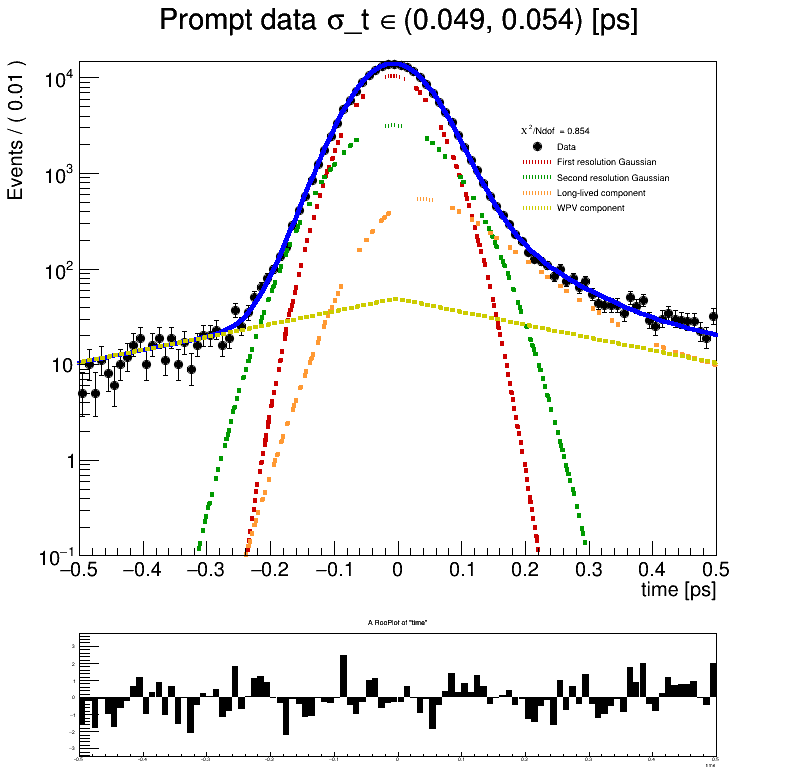
\includegraphics[width=\textwidth]{gpx/total_pdf_fit_zoom_b6.pdf}
    \end{column}
  \end{columns}

\pdfnote{Putting everythin toguether we have the resolution pdf}
\pdfnote{In the right side, we can see all the components involved in the extraction of the resolution. this picture corresponds to 2017 at the 6th bin}

\end{frame} % ------------------------------------------------------------------
  
  

\subsection{{\color{red}WIP:} Calibrating the decay-time resolution}
\begin{frame}[default] % -------------------------------------------------------
\frametitle{noframetitle}

\begin{columns}%[T]
  \begin{column}{0.475\textwidth}
      \begin{itemize}
        \item We use an effective single-Gaussian resolution for easier calculation of the systematic uncertainties.
        \begin{block}{Effective resolution}
          {\small $$ \sigma_{\text{eff}} = \sqrt{ \frac{-2}{\Delta m_s^2} \text{log} \left(\sum_{i=1}^2 f_i e^{-\sigma_i^2 \frac{\Delta m_s^2}{2}} \right) }$$ }
        \end{block}
        
        \item Then the calibration is obtained by a 10-points linear fit to $\sigma_{\text{eff}}$
      \end{itemize}
  \end{column}
  \begin{column}{0.475\textwidth}
    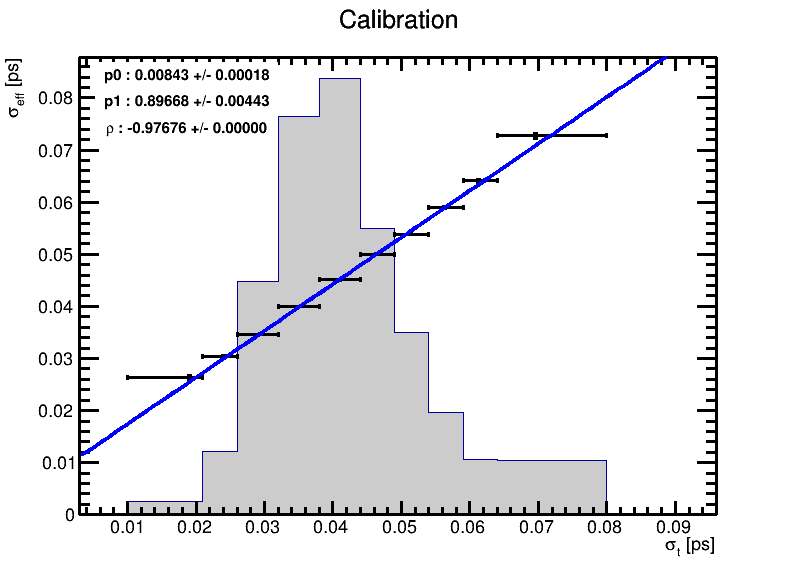
\includegraphics[width=\textwidth]{gpx/resolution_plot.pdf}
 \end{column}
\end{columns}

\pdfnote{After we extract the resolution we need to calibrate it. When introducing resolution in the final pdf we use an effective single gaussian, since it is easier to implement and also is easier for the calculation of systematic uncertainties.}
\pdfnote{The calibration is finally obtained from a 10 points linear fit to the effective resolution as we can see at the right hand side ot htis slide}

\end{frame} % ------------------------------------------------------------------


\subsection{{\color{red} WIP:} VELO alignment bias}
\begin{frame}[default] % -------------------------------------------------------
\frametitle{noframetitle}
\begin{itemize}
  \item Decay time (negative) bias seen in prompt samples used for time resolution studies in $B_s^0 \rightarrow J/\psi \phi$ and $B_s^0 \rightarrow D_s h$ using Run 2 data.
  \item Produced by a VELO misalignment which reflects in biased measured decay length.
  \item We know it could affect $\Gamma_s$ and $\Delta m_s$ measurements. 
\end{itemize}

\begin{columns}%[T]
  \begin{column}{0.475\textwidth}
    \begin{block}{First solution}
      \begin{itemize}
      \item Study this effect in $J/\psi$ prompt samples.
      \item Realign VELO.
      \end{itemize}
    \end{block}
    \begin{block}{What has been done}
      \begin{itemize}
      \item Confirm the existence of the bias: look at all 2017 MagUp using DIMUON stream.
      \item Try refitting the candidates and the PVs and see if it gets better. 
    \end{itemize}
    \end{block}
  \end{column}
  \begin{column}{0.475\textwidth}
    \begin{center}
      \footnotesize 2017 MagUp data \vspace*{-2mm}
    \end{center}
    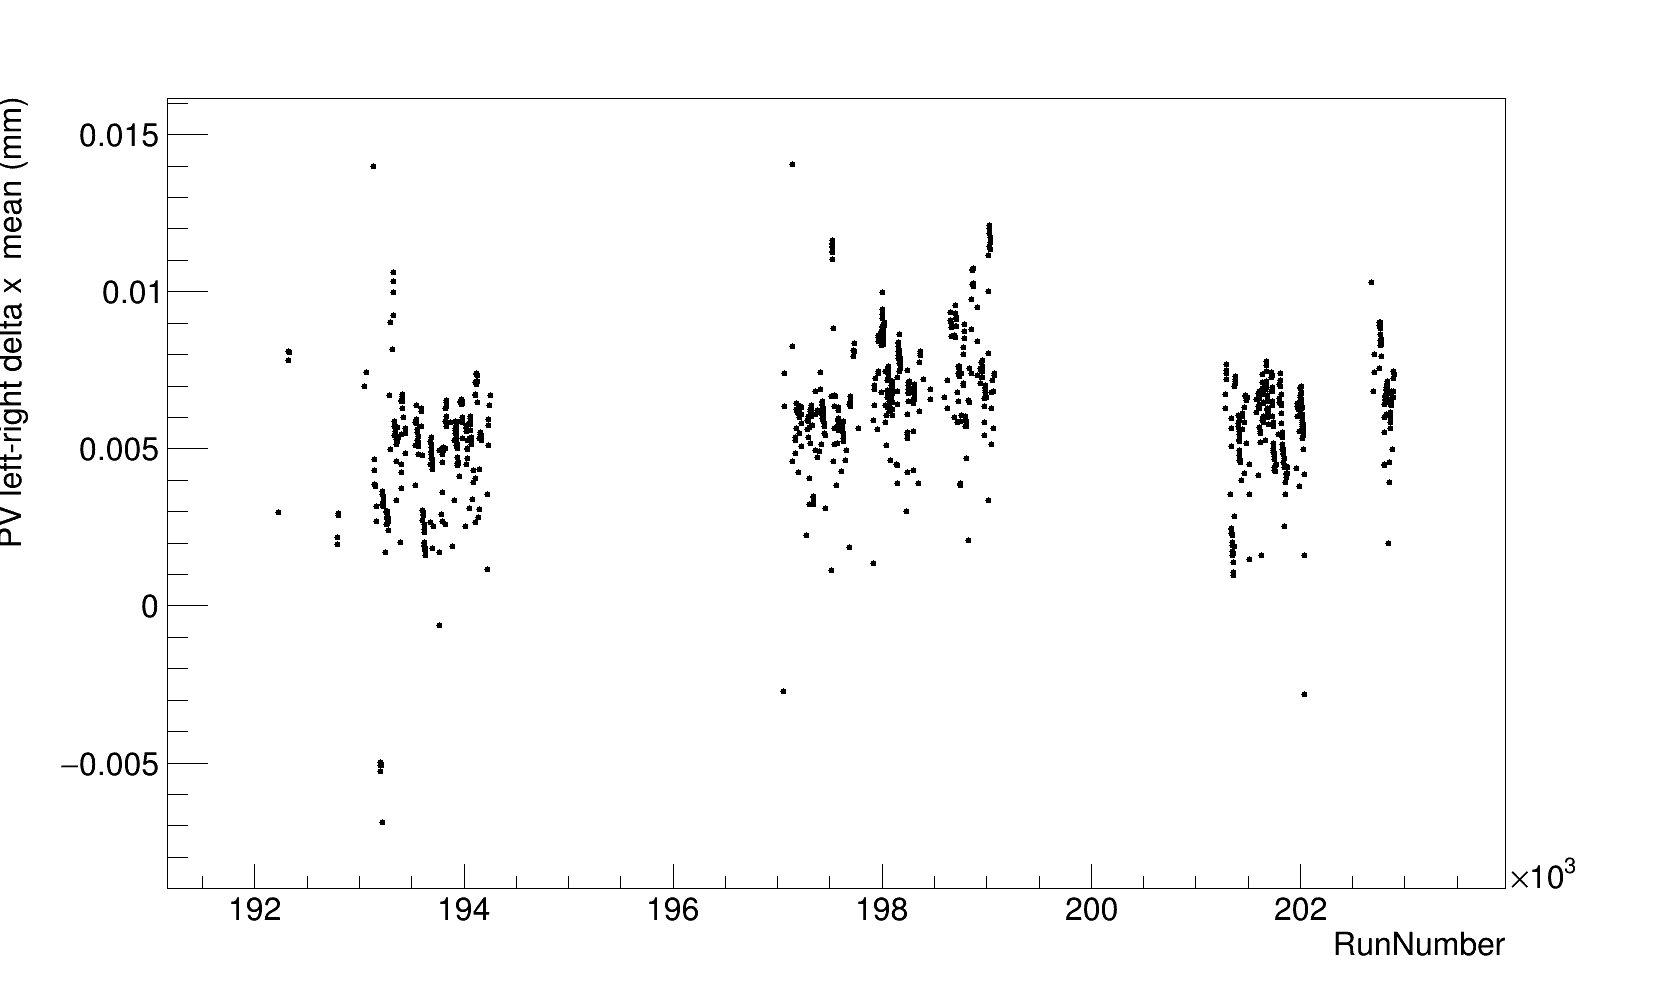
\includegraphics[width=\textwidth]{gpx/JpsiPhiBiasTitles.png}
  \end{column}
\end{columns}

\pdfnote{A few notes on the recently VELO alignment bias. A negative decay time bias has been observer in prompt sampels uses for time resolution studies in Bs2JpsiPhi asn Bs2Ds hadron. This is due to a VELO misalignment which is reflected in biased measured decay time lengh. This could affect our Gs and DMs measurements}

\pdfnote{The first attempt to solve this issue, consists in studying this effect in J/psi prompt samples and try to realign the VELO}

\pdfnote{What is already done is that we have confiemer the existence of the biased looking at all 2017 magnet up using dimuon streams, that are known to be one of the worst runs. As we can see on the picture on the right, which shows the left right delta x vs the run number. Currently we are working on refitting the canditates and de PVs and see if it gets better}

\end{frame} % ------------------------------------------------------------------



\section{Decay--time acceptance}



\subsection{Procedure}
\begin{frame}[default] % -------------------------------------------------------
\frametitle{noframetitle}

\begin{columns}[T]
  \begin{column}{0.5\textwidth}
    \begin{itemize}
      %\item Data-driven decay-time acceptance
      \item We use $B_d^0 \rightarrow J/\psi K^* [K^+ \pi^-]$ as control channel
      \item We effectively measure $\Gamma_s - \Gamma_d$ 
      %\item Simultaneous fit to three datasets
      \begin{description}[bddata]
        \item[$B_s^0$ MC] We fit {\footnotesize $\varepsilon_{\text{MC}}^{B_s^0}[t] \times \text{exp}\left(\Gamma_{s}^{\text{gen}} t\right) \otimes \text{exp}\left(\frac{-t^2}{{2\sigma_{MC}^{B_s}}^2}\right)$}.
        \item[$B_d^0$ MC] We fit {\footnotesize $\varepsilon_{\text{MC}}^{B_d^0}[t] \times \text{exp}\left(\Gamma_{d}^{\text{gen}} t\right) \otimes \text{exp}\left(\frac{-t^2}{{2\sigma_{MC}^{B_s}}^2}\right)$}.
        \item[$B_d^0$ data] We fit {\footnotesize $\varepsilon_{\text{data}}^{B_d^0}[t] \times \text{exp}\left(\Gamma_{d}^{\text{WA}} t\right) \otimes \text{exp}\left(\frac{-t^2}{{2\sigma_{data}^{B_d}}^2}\right)$}.
      \end{description} in two trigger categories (and per year).
      \item Hence $B_s^0$ data decay-time acceptance is 
      $$ \varepsilon_{\text{data}}^{B_s^0} = \varepsilon_{\text{data}}^{B_d^0}[t] \times \frac{ \varepsilon_{\text{MC}}^{B_s^0}[t] }{ \varepsilon_{\text{MC}}^{B_d^0}[t] }.$$
    \end{itemize}
  \end{column}
  
  \begin{column}{0.5\textwidth}
    \vspace*{-2mm}
    \includegraphics[width=\columnwidth]{gpx/reweighting_pipeline.pdf}
    \vspace*{-2mm}
      \begin{itemize}
        \item $B_{s,d}^0$ MC are reweigthed to $B_{s,d}^0$ data in polarity.
        \item $B_{s,d}^0$ MC are reweigthed to $B_{s,d}^0$ data to account for the S-wave.
        \item $B_{d}^0$ data is reweigthed to $B_{s}^0$ data to match $p_T(B)$ and $p(B)$ distributions
        \item $B_{s,d}^0$ MC are reweigthed to $B_{s,d}^0$ data to match $p_T(B)$ and $m(KK),m(K\pi)$ distributions
      \end{itemize}
    \end{column}
\end{columns}

\pdfnote{Concerning decay time acceptance, the procedure is in place, and we are now dealing with the validation tests}
\pdfnote{So, basically we use Bd2JpsiKstar as our control channel since it has a DG=0, hence the time dependent part factorices from the angular one. To do som we use 3 splines that model the decay time acceptance. Each of the splies models the efficiency from a different datsset BsMC, BdMC and BdData. These 3 splines are combined as in the bottom expression to finally get the efficiency in Bs data}
\pdfnote{The splines are multipliying a exponential convoluted with a gaussiand of meand 0 and sigma equal to the resolution}
\pdfnote{Though Bd and Bs decays are kinematically similar, we correct differences via some reweightings, following the pipeline at top right. Both Bs and Bd MC are reweighted to their corresponding data in polarity. Since our MCs dont account for Swave we reweight them to have it. Bd data is GB-reweightied to Bs data in p and pT, and finally MC are reweighted to their corresponding data samples in pT and the phi or kstar mass}

\end{frame} % ------------------------------------------------------------------



\subsection{Spline basis}
\begin{frame}[default] % -------------------------------------------------------
\frametitle{noframetitle}

\begin{columns}%[T]
  \begin{column}{0.6\textwidth}
    \begin{itemize}
      \item Efficiency is modelled with cubic b-splines.
      \item Basis fixed with a set of knots, $k$, $$k = \{0.3, 0.58, 0.91, 1.35, 1.96, 3.01,7.00\}$$
      \vspace*{-3mm}
      \item For a spline with $6+1$ knots, we have to fit $8$ coefficients.
      \begin{itemize}
        \item Set of 9 coefficients $\{c_i\}_{i=0}^{8}$.
        \item Normalization condition: $c_0=1$.
        \item For a given bin, the spline is $$  s[t] = b_0 + b_1 t + b_2 t^2 + b_3 t^3. $$
        \item Each $b_i = b_i(t,c)$, are indeed functions of $c$ coefficients,
        \item At the last knot, a linear extrapolation is done up to $t = 15$ ps.
      \end{itemize}
    \end{itemize}
  \end{column}
  \begin{column}{0.35\textwidth}
    \includegraphics[width=\textwidth]{gpx/splinecolors.pdf}
    \includegraphics[width=\textwidth]{gpx/interesting.pdf}
  \end{column}
\end{columns}

\pdfnote{Digging a bit in how these splines are built, first thing is they actually are b-spline, so they need a basis. We fix it with a set of knots wich we exponentialy distibute from 0.3 to 15 ps (last knot is moved to 7ps because of very low statistics in that bin)}
\pdfnote{For s spline of 6+1 knots, we have to fit 8 coefficients since the first one can be fixed to 1 as a normalization condition. In each bin, the spline has the form third degree polynomial we see here, where each b coefficient is actually function of the c coefficients depending in which time bin the event lies on}
\pdfnote{A linear extrapolation is done up to 15 ps. We can see at top right a how a efficiency is build from each of the bsplines. And at bottom right, a exponential convoluted with a gaussian times a spline is shown for ilustration purposes.}

\end{frame} % ------------------------------------------------------------------



\subsection{Latest results}
\begin{frame}[default] % -------------------------------------------------------
\frametitle{noframetitle}

\begin{tabular}{rcccc}
       & 2015 & 2016 & 2017 & 2018 \\ 
biased & 
\includegraphics[width=0.2\textwidth]{../output/figures/time_acceptance/2015/Bd2JpsiKstar/v0r5_simul_biased_spline.pdf} & 
\includegraphics[width=0.2\textwidth]{../output/figures/time_acceptance/2016/Bd2JpsiKstar/v0r5_simul_biased_spline.pdf} & 
\includegraphics[width=0.2\textwidth]{../output/figures/time_acceptance/2017/Bd2JpsiKstar/v0r5_simul_biased_spline.pdf} & 
\includegraphics[width=0.2\textwidth]{../output/figures/time_acceptance/2018/Bd2JpsiKstar/v0r5_simul_biased_spline.pdf} \\
& \\
unbiased & 
\includegraphics[width=0.2\textwidth]{../output/figures/time_acceptance/2015/Bd2JpsiKstar/v0r5_simul_unbiased_spline.pdf} & 
\includegraphics[width=0.2\textwidth]{../output/figures/time_acceptance/2016/Bd2JpsiKstar/v0r5_simul_unbiased_spline.pdf} & 
\includegraphics[width=0.2\textwidth]{../output/figures/time_acceptance/2017/Bd2JpsiKstar/v0r5_simul_unbiased_spline.pdf} & 
\includegraphics[width=0.2\textwidth]{../output/figures/time_acceptance/2018/Bd2JpsiKstar/v0r5_simul_unbiased_spline.pdf} \\
\end{tabular}

\pdfnote{Here we shown real life splines for all years or Run2 in both trigger categories. These are our latest time accpentaces, where we can see that most of our statistics comes from unbiased events just by looking at 1sigma confidence bands}

\end{frame} % ------------------------------------------------------------------





\subsection{Validation}
\begin{frame}[default] % -------------------------------------------------------
\frametitle{noframetitle}

  \begin{itemize}
    \item Strategy validation
    \begin{description}[lifetimeBBB]
      \item[$B^+$ lifetime] Using $B^+ \rightarrow J/\psi K^+$ channel and $B_0 \rightarrow J/\psi K^*$ as control channel:
      \begin{enumerate}
        \item Swap $B_s^0$ MC with $B^+$ MC and compute acceptance.
        \item Fit $B^+$ data sample with that acceptance obtaining $\tau_{B^+}/\tau_{B^0}$.
      \end{enumerate}
      \item[$B^0$ lifetime] Split $B_0$ samples in two halves, one as control channel.
      \begin{enumerate}
        \item Compute acceptance with first half (take $\tau_{B_d} = 1.520$ ps).
        \item Fit second half with that acceptance obtaining $\tau_{B^0}$.
      \end{enumerate}
    \end{description}
    \item Procedure validation
    \begin{itemize}
      \item Fit MC ${\small \Delta \Gamma \neq 0}$, previously weighting $\Delta \Gamma \neq 0$ MC to be like $\Delta \Gamma = 0$.
      \item Repeat the procedure with different set of knots
    \end{itemize} 
  \end{itemize}


\pdfnote{Finishing with the time accepntace, just a brief summary of the validation we have still to do}
\pdfnote{First, Concerning the validtation of the Strategy, we compute B+ and B0 lifetimes}
\pdfnote{Secondly, a procedure Validation is done. This is already implemented, whilst the Strategy is currently ongoing}

\end{frame} % ------------------------------------------------------------------




\subsection{IPchi2 bias}
\begin{frame}[default] % -------------------------------------------------------
\frametitle{noframetitle}

We should not be affected by the $\chi_{IP}^2$ bias.

\vfill

\begin{tabular}{rccc}
  & $B_s^0$ data to MC & $B_d^0$ data to MC & $B_d^0$ data to $B_s^0$ data\\
  $\mathsf{log} \, \chi_{nDoF}^2 (B)$ &
  \includegraphics[width=0.25\textwidth]{gpx/log_B_DTF_CHI2NDOF_Bs2017.pdf} &
  \includegraphics[width=0.25\textwidth]{gpx/log_B_DTF_CHI2NDOF_Bd2017.pdf} &
  \includegraphics[width=0.25\textwidth]{gpx/log_B_DTF_CHI2NDOF_BsBd2017.pdf} \\
  $\mathsf{log} \, \chi_{IP}^2 (B)$ & 
  \includegraphics[width=0.25\textwidth]{gpx/log_B_IPChi2_Bs2017.pdf} &
  \includegraphics[width=0.25\textwidth]{gpx/log_B_IPChi2_Bd2017.pdf} &
  \includegraphics[width=0.25\textwidth]{gpx/log_B_IPChi2_BsBd2017.pdf} \\
\end{tabular}

\pdfnote{here just a slide on IPchi2 bias. We are not affecte by this bias as we can see from the plots. Above all, our time accpentace and resolution effects are calibrated from data, so we should be fine here.}
\pdfnote{velo hit resolution affects track parameters: everything that relies on velo hit resolution to be the same in data and MC is affected}

\end{frame} % ------------------------------------------------------------------
  
  

\section{Angular acceptance}



\subsection*{Procedure}
\begin{frame}[default] % -------------------------------------------------------
\frametitle{noframetitle}

\begin{columns}[T]
  \begin{column}{0.27\textwidth}
    \begin{enumerate}
      \item Naive angular weights.
      \item Polarity and kinematic weightings to correct MC to match data shape.
      \item Corrected angular weights.
      \item Perform a time--angular fit to data and use fitted parameters to weight the MC.
      \item Weight $K^+$ and $K^-$ momentum and transverse momentum distributions.
      \item Corrected angular weights.
    \end{enumerate}

  \end{column}
  \begin{column}{0.7\textwidth}
    \begin{center}
      \centering \includegraphics[width=\textwidth]{gpx/angular_pipeline.pdf}
    \end{center}

    \begin{columns}
      \begin{column}{0.45\textwidth}
        \begin{variableblock}{Iterative procedure}{bg=scqred!20}{bg=scqred}
          We iterate steps 4-5-6 until we get the procedure to converge.
        \end{variableblock}
      \end{column}
      \begin{column}{0.35\textwidth}
        \begin{variableblock}{Convergence}{bg=gray!20}{bg=gray}
          Usually it takes 4-6 iterations to converge.
        \end{variableblock}
      \end{column}
    \end{columns}
  \end{column}
\end{columns}

\pdfnote{We get to the angular acceptance, which is an expensive procedure.}
\pdfnote{We can divide it in to parts: the setup and the iterative procedure.}
\pdfnote{In the setup part we have steps 1 and 2. Fisrt a very naive set of angular acceptance weights is computed, were we basically divide our time angular dependent pdf by our time dependent and that times the angular functions. Then we start correcting MC as before: polarity and kinematic GB-weighting. And we compute the correclted angular weights that are the starting point of the iterative procedure}
\pdfnote{We use those angular weights as input for ar time-angular dependent fit (like the final one wher we extract our main parameters), the we apply pdf weights to correct MC to have S wave using those main parameters. After that we GB-reweight MC to data in both p and pT of the kaons, and finally we compute the fully corected set of angular accpentace weights at the first iteration.}

\end{frame} % ------------------------------------------------------------------


\subsection*{Latest results}
\begin{frame}[default] % -------------------------------------------------------
\frametitle{noframetitle}

  \begin{columns}
    \begin{column}{0.55\textwidth}
      \begin{itemize}
        \item We apply ${}_s$Weights, so we only need to model efficient in signal efficiency.
        \item As an example, the 2016 angular acceptance is shown in this table (pictures ilustrate the same acceptances)
        \begin{tabular}{c|r@{$\pm$}l|r@{$\pm$}l}
          & \multicolumn{2}{c|}{biased} & \multicolumn{2}{c}{unbiased} \\ \hline
          $ w_{00} $&$      1.0 $&$ 0.0       $&$      1.0 $&$ 0.0      $  \\
          $ w_{\parallel \parallel} $&$   1.0251 $&$  0.0015 $&$  1.03393 $&$ 0.00067$  \\
          $ w_{\perp \perp} $&$   1.0250 $&$  0.0014 $&$  1.03353 $&$ 0.00066$  \\
          $ w_{\perp \parallel} $&$   0.0025 $&$  0.0012 $&$ -0.00075 $&$ 0.00053$  \\
          $ w_{0 \parallel} $&$  0.00305 $&$ 0.00069 $&$  0.00036 $&$ 0.00032$  \\
          $ w_{0 \perp} $&$ -0.00033 $&$ 0.00069 $&$  0.00021 $&$ 0.00032$  \\
          $ w_{SS} $&$   1.0143 $&$  0.0010 $&$  1.00861 $&$ 0.00046$  \\
          $ w_{S\parallel} $&$ -0.00006 $&$ 0.00089 $&$  0.00028 $&$ 0.00041$  \\
          $ w_{S\perp} $&$  0.00008 $&$ 0.00090 $&$  0.00010 $&$ 0.00042$  \\
          $ w_{S0} $&$  -0.0003 $&$  0.0019 $&$ -0.00243 $&$ 0.00086$  \\
        \end{tabular}
        \item To validate the procedure we use $B^0 \rightarrow J/\psi K^* $ data
      \end{itemize} 
    \end{column}

    \begin{column}{0.4\textwidth}
      \begin{tabular}{c|c}
        biased & unbiased \\ \hline
        \includegraphics[width=0.45\textwidth]{gpx/2016_BiasedTrig_AngAcc_Baseline_Iteration6_eff_cos_psi_fit.pdf}
        &
        \includegraphics[width=0.45\textwidth]{gpx/2016_UnbiasedTrig_AngAcc_Baseline_Iteration6_eff_cos_psi_fit.pdf} 
        \\
        \includegraphics[width=0.45\textwidth]{gpx/2016_BiasedTrig_AngAcc_Baseline_Iteration6_eff_cos_theta_fit.pdf} 
        &
        \includegraphics[width=0.45\textwidth]{gpx/2016_UnbiasedTrig_AngAcc_Baseline_Iteration6_eff_cos_theta_fit.pdf}
        \\
        \includegraphics[width=0.45\textwidth]{gpx/2016_BiasedTrig_AngAcc_Baseline_Iteration6_eff_phi_fit.pdf} 
        &
        \includegraphics[width=0.45\textwidth]{gpx/2016_UnbiasedTrig_AngAcc_Baseline_Iteration6_eff_phi_fit.pdf} 
      \end{tabular}
    \end{column}
  \end{columns}

\pdfnote{Here I show you some of our latest results, as a matter of fact, 2016 ones. I the table we can see how the angular accpetance weights look like. Basically they are one when the amplitude interferes with itself, and zero otherwise}
\pdfnote{Almost everithing in place but the valitation with B0 data, with in Currently ongoing}
\pdfnote{At right hand side we see these efficiencie ploted. These are just for ilustration, since we do not use legende polunomials to modell the acceptance. Here fourth-order polynomial parameterisation of each one-dimensional efficiency is used}

\end{frame} % ------------------------------------------------------------------



\section{Hyperthreading}



\begin{frame}[default] % -------------------------------------------------------
\frametitle{nosubsection}

\begin{center}
  \includegraphics[scale=0.32]{gpx/CPUioGPU.pdf}
\end{center}

\begin{multicols}{2}
  \begin{itemize}
    \item \texttt{ipanema3} allow us to use both cuda-C and openCL to run this analysis in
    any parallel device and also on multi-core CPU. \vfill
    \item Both time and angular acceptances are now running under \texttt{ipanema3}. 
    \item Per event parallelization reduces fitting time about a $\times 10$ factor.
    \item Likelihood profile scans and most of the generated toyMCs (for systematic studies) were done with ipanema.
  \end{itemize}
\end{multicols}

\pdfnote{Here I want to show a slide about how these computations are beeing done. The phis team in Santiago develop a gpu-based calculation of both time and angular accepntaces. }
\pdfnote{To do so, we use ipanema3 which is a python package, which plays the go-between role here betwen the user and the gpu device.}

\end{frame} % ------------------------------------------------------------------



\section{Preliminary fit results}



\begin{frame}[default] % -------------------------------------------------------
\frametitle{nosubsection}

\begin{itemize}
  \item Currently we are repeating all the tests as in the previous round.
  \item $\phi_s$ and $\Delta \Gamma$ are blinded.
\end{itemize}

\begin{center}
\begin{columns}[T]
  \begin{column}{0.3\textwidth}
      \centering
      \begin{variableblock}{Main parameters}{bg=scqblue!20}{bg=scqblue}
      \begin{tabular}{cr@{\pm}l}
      $\phi_0(*)                       $    & $     0.293$ & $    0.021$  \\
      $\lambda_0                       $    & $    1.0066$ & $   0.0096$  \\
      $f_0                             $    & $    0.5180$ & $   0.0017$  \\
      $f_{\perp}                       $    & $    0.2462$ & $   0.0023$  \\
      $\delta_{\parallel} - \delta_0   $    & $     3.131$ & $    0.061$  \\
      $\delta_{\perp} - \delta_0       $    & $     2.768$ & $    0.072$  \\
      $\Delta\Gamma_s(*)               $    & $    0.2671$ & $   0.0044$  \\
      $\Gamma_s - \Gamma_d             $    & $   -0.0086$ & $   0.0013$  \\
      $\Delta m                        $    & $    17.739$ & $    0.032$  \\
    \end{tabular}
    \end{variableblock}
  \end{column}
  \begin{column}{0.3\textwidth}
    \centering
    \begin{variableblock}{S-wave parameters}{bg=scqorange!20}{bg=scqorange}
      \begin{tabular}{cr@{\pm}l}
      $f_S^{1}                         $    & $     0.467$ & $    0.024$  \\
      $f_S^{2}                         $    & $    0.0417$ & $   0.0049$  \\
      $f_S^{3}                         $    & $    0.0033$ & $   0.0014$  \\
      $f_S^{4}                         $    & $    0.0042$ & $   0.0025$  \\
      $f_S^{5}                         $    & $    0.0551$ & $   0.0071$  \\
      $f_S^{6}                         $    & $     0.151$ & $    0.011$  \\
      $\delta_S^{1} - \delta_{\perp}   $    & $      2.03$ & $     0.13$  \\
      $\delta_S^{2} - \delta_{\perp}   $    & $      1.71$ & $     0.18$  \\
      $\delta_S^{3} - \delta_{\perp}   $    & $      1.00$ & $     0.31$  \\
      $\delta_S^{4} - \delta_{\perp}   $    & $     -0.16$ & $     0.12$  \\
      $\delta_S^{5} - \delta_{\perp}   $    & $    -0.601$ & $    0.066$  \\
      $\delta_S^{6} - \delta_{\perp}   $    & $    -0.990$ & $    0.077$  \\
      \end{tabular}
      \end{variableblock}
    \end{column}
\end{columns}
\end{center}

\pdfnote{And to end this talk here you have a sneak peek of the Preliminary results of the full run2 analysis. Currently we are repeating all the test in bins of variables, per year etc. In this blocks you can see the statistical uncertainty LHCb will achieve in phis.}

\end{frame} % ------------------------------------------------------------------








\begin{frame}[plain,backgroundpicture=gpx/aiandes.pdf,overlaytoc=0.9]
  \addtocounter{framenumber}{-1}
  \hspace*{5.3cm}
  \vspace*{-3.3cm}
  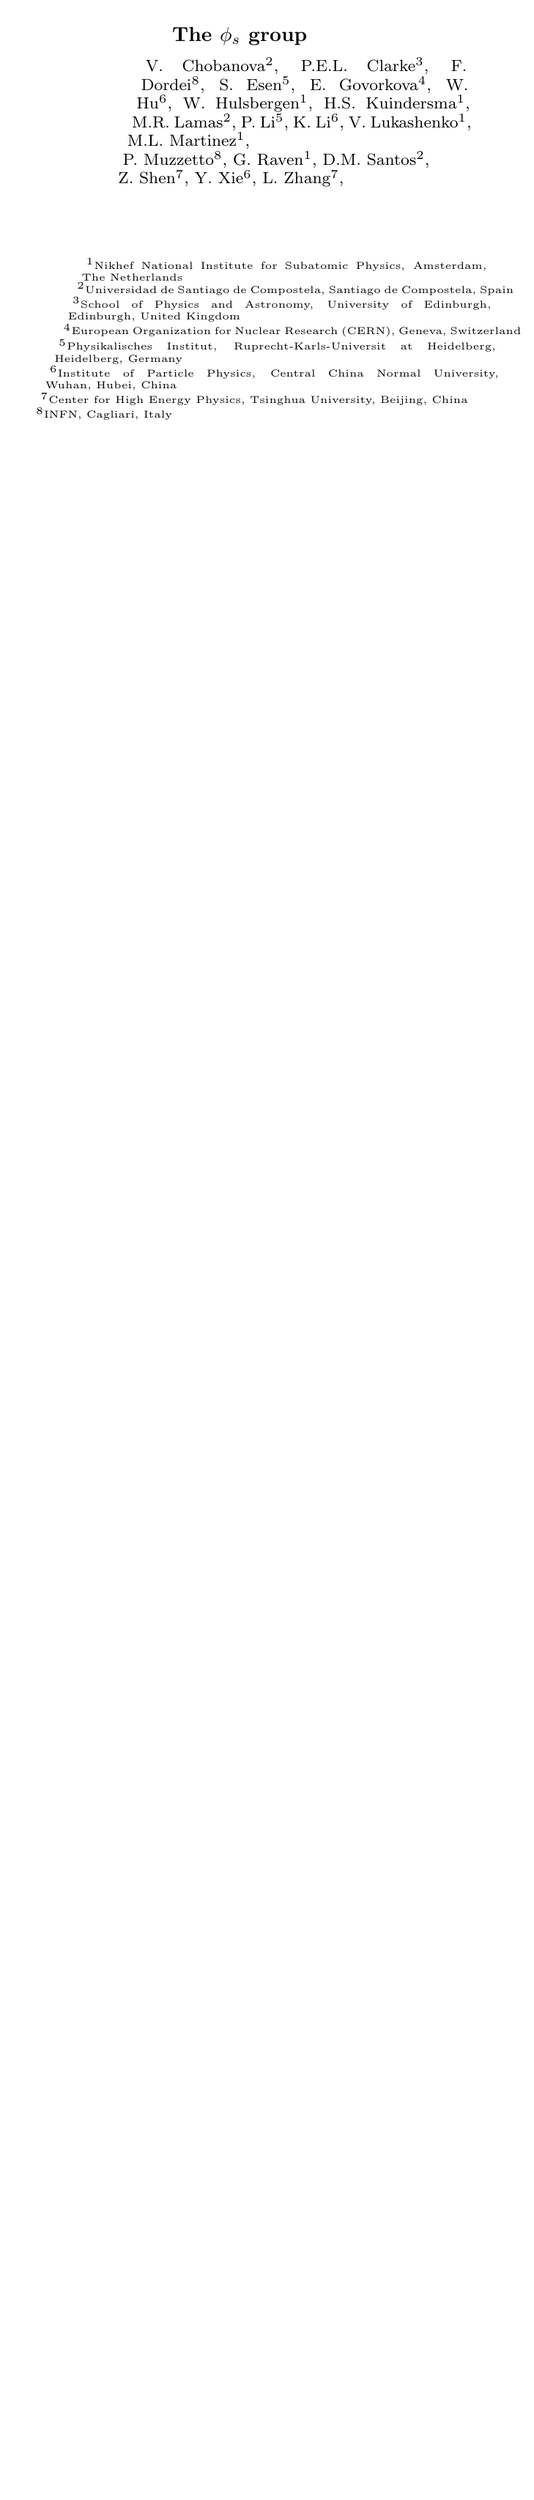
\begin{tikzpicture}
    \node[anchor=south west,xshift=-2cm] at (0,0) {
      \begin{minipage}{0.99\textwidth} 
        \Shapepar{\myparshape}
        %
        \textbf{The $\phi_s$ group}\\
          \phantom{caca}\footnotesize \\
          V. Chobanova$^2$,
          P.E.L. Clarke$^3$,
          F. Dordei$^8$,
          S. Esen$^5$,
          E. Govorkova$^4$,
          W. Hu$^6$,
          W. Hulsbergen$^1$,
          H.S. Kuindersma$^1$,
          M.R. Lamas$^2$, 
          P. Li$^5$,
          K. Li$^6$,
          V. Lukashenko$^1$,
          M.L. Martinez$^1$,\\
          P. Muzzetto$^8$,
          G. Raven$^1$,
          D.M. Santos$^2$,\\
          Z. Shen$^7$,
          Y. Xie$^6$,
          L. Zhang$^7$,
          \phantom{cacaca}\\
          \phantom{cacaca}\\
          \phantom{cacaca}\\
          \phantom{cacaca}\\
          \phantom{cacaca}\\
          \phantom{cacaca}\\
          \phantom{cacaca}\\
          %
          %
          \tiny
          $ ^1$Nikhef National Institute for Subatomic Physics, Amsterdam, The Netherlands\\
          $ ^2$Universidad de Santiago de Compostela, Santiago de Compostela, Spain\\
          $ ^3$School of Physics and Astronomy, University of Edinburgh, Edinburgh, United Kingdom\\
          $ ^4$European Organization for Nuclear Research (CERN), Geneva, Switzerland\\
          $ ^5$Physikalisches Institut, Ruprecht-Karls-Universit at Heidelberg, Heidelberg, Germany\\
          $ ^6$Institute of Particle Physics, Central China Normal University, Wuhan, Hubei, China\\
          $ ^7$Center for High Energy Physics, Tsinghua University, Beijing, China\\
          $ ^8$INFN, Cagliari, Italy\\
          \phantom{$ ^9$School of Physics State Key Laboratory of Nuclear Physics and Technology, Peking University, Beijing,China}
      \end{minipage}
    };
  \end{tikzpicture}
\end{frame}
%\phantom{\section{Backup}}
\section*{Backup}


\subsection*{Differencial cross-rate}
\begin{frame}[default] % -------------------------------------------------------
\frametitle{noframetitle}

\begin{eqnarray*}
  \frac{d^4 \Gamma( t) }{ d\cos\theta_K d\cos\theta_l d\phi}&=&  \sum_{k=1}^{10} N_k h_k(t) f_k(\theta_K, \theta_l, \phi),  
  \end{eqnarray*}
 where the decay-time-dependent functions $h_k(t)$ are given as
 \begin{eqnarray*}
  h_k^{B_s^0}(t)= \frac{3}{ 4\pi}
    e^{-\Gamma t}\left\{ a_k \cosh\frac{\Delta \Gamma t}{2} + b_k \sinh\frac{\Delta \Gamma t}{2} + c_k \cos(\Delta mt)  +  d_k \sin(\Delta mt) \right\}, \\
  h_k^{\overline{B}_s^0}(t)= \frac{3}{ 4\pi}
    e^{-\Gamma t}\left\{ a_k \cosh\frac{\Delta \Gamma t}{2} + b_k \sinh\frac{\Delta \Gamma t}{2} - c_k \cos(\Delta mt)  -  d_k \sin(\Delta mt) \right\}.
 \end{eqnarray*}
 

\end{frame} % ------------------------------------------------------------------



\begin{frame}[default] % -------------------------------------------------------
\frametitle{Coefficients}

\centering 
\resizebox{0.8\textwidth}{!}{%
\begin{tabular}[t]{c|c|c|c |ccc}
\toprule
  $f_k$ & $N_k$ &  $a_k$ & $b_k$ & $c_k$ & $d_k$ \\
  \midrule
  %%%%%%%%%%%%%
  $ c^2_K s^2_l $
  & $ |A_0|^2     $
  & $\frac{1}{2}(1+ |\lambda_{0}|^2)$
  & $-|\lambda_0| \cos(\phi_0) $
  & $\frac{1}{2}(1-|\lambda_{0}|^2)$
  & $ |\lambda_0| \sin(\phi_0)$ \\
  \hline
  %%%%%%%%%%%%%
  $ \frac{1}{2}{s^2_K (1- c_\phi^2 s_l^2)} $
  & $ |A_{||}|^2$
  & $\frac{1}{2}(1+ |\lambda_{{||}}|^2)$
  & $-|\lambda_{{||}}| \cos(\phi_{{||}}) $
  & $\frac{1}{2}(1-|\lambda_{{||}}|^2)$
  & $ |\lambda_{{||}}| \sin(\phi_{{||}})$ \\
  \hline
  %%%%%%%%%%%
  $ \frac{1}{2}s^2_K (1- s_\phi^2 s_l^2) $
  & $|A_{\perp} |^2 $
  & $\frac{1}{2}(1+ |\lambda_{{\perp}}|^2)$
  & $|\lambda_{{\perp}}| \cos(\phi_{{\perp}}) $
  & $\frac{1}{2}(1-|\lambda_{{\perp}}|^2)$
  & $ -|\lambda_{{\perp}}| \sin(\phi_{{\perp}})$ \\
  \hline
  %%%%%%%%%%
  $  s^2_K   s_l^2  s_\phi c_\phi  $
  &  $  |A_{\perp} A_{||}|$
  &  $\begin{array}{l}
    \frac{1}{2} \bigg[\sin (\delta_{\perp}-\delta_{||})  - |\lambda_{\perp}  \lambda_{||} |\\  \sin( \delta_{\perp}-\delta_{||} -\phi_{\perp} +\phi_{||})   \bigg]
  \end{array}$
  &  $\begin{array}{l}
    \frac{1}{2} \bigg[ |\lambda_{\perp}| \sin (\delta_{\perp}-\delta_{||} -\phi_{\perp}) \\    + | \lambda_{||} |\sin( \delta_{||}-\delta_{\perp}  -\phi_{||})   \bigg]
  \end{array}$
  & $\begin{array}{l}
    \frac{1}{2} \bigg[\sin (\delta_{\perp}-\delta_{||})  + |\lambda_{\perp}  \lambda_{||} |\\  \sin( \delta_{\perp}-\delta_{||} -\phi_{\perp} +\phi_{||})   \bigg]
  \end{array}$
  &  $\begin{array}{l}
    -\frac{1}{2} \bigg[ |\lambda_{\perp}| \cos (\delta_{\perp}-\delta_{||} -\phi_{\perp}) \\    + | \lambda_{||} |\cos( \delta_{||}-\delta_{\perp}  -\phi_{||})   \bigg]
  \end{array}$    \\
  \hline
  %%%%%%%
  $\sqrt 2 s_K c_K s_l c_l c_\phi   $
  &  $|A_{0} A_{||}|$
  &  $\begin{array}{l}
    \frac{1}{2} \bigg[\cos (\delta_{0}-\delta_{||})  + |\lambda_{0}  \lambda_{||} |\\  \cos( \delta_{0}-\delta_{||} -\phi_{0} +\phi_{||})   \bigg]
  \end{array}$
  &  $\begin{array}{l}
    -\frac{1}{2} \bigg[|\lambda_{0}|\cos (\delta_{0}-\delta_{||}-\phi_0 )  \\  + | \lambda_{||} |\cos( \delta_{||}-\delta_{0} -\phi_{||})   \bigg]
  \end{array}$
  &  $\begin{array}{l}
    \frac{1}{2} \bigg[\cos (\delta_{0}-\delta_{||})  - |\lambda_{0}  \lambda_{||} |\\  \cos( \delta_{0}-\delta_{||} -\phi_{0} +\phi_{||})   \bigg]
  \end{array}$
  &  $\begin{array}{l}
    -\frac{1}{2} \bigg[|\lambda_{0}|\sin (\delta_{0}-\delta_{||}-\phi_0 )  \\  + | \lambda_{||} |\sin( \delta_{||}-\delta_{0} -\phi_{||})   \bigg]
  \end{array}$ \\
  \hline
%%%%%%%%
  $ -\sqrt 2 s_K c_K s_l c_l s_\phi  $
  &  $|A_{0} A_{\perp}|$
  &  $\begin{array}{l}
    -\frac{1}{2} \bigg[\sin (\delta_{0}-\delta_{\perp})  - |\lambda_{0}  \lambda_{\perp} |\\  \sin( \delta_{0}-\delta_{\perp} -\phi_{0} +\phi_{\perp})   \bigg]
  \end{array}$
  &  $\begin{array}{l}
    \frac{1}{2} \bigg[ |\lambda_{0}| \sin (\delta_{0}-\delta_{\perp} -\phi_{0}) \\    + | \lambda_{\perp} |\sin( \delta_{\perp}-\delta_{0}  -\phi_{\perp})   \bigg]
  \end{array}$
  & $\begin{array}{l}
    -\frac{1}{2} \bigg[\sin (\delta_{0}-\delta_{\perp})  + |\lambda_{0}  \lambda_{\perp} |\\  \sin( \delta_{0}-\delta_{\perp} -\phi_{0} +\phi_{\perp})   \bigg]
  \end{array}$
  &  $\begin{array}{l}
    -\frac{1}{2} \bigg[ |\lambda_{0}| \cos (\delta_{0}-\delta_{\perp} -\phi_{0}) \\    + | \lambda_{\perp} |\cos( \delta_{\perp}-\delta_{0}  -\phi_{\perp})   \bigg]
  \end{array}$    \\
  \hline
  %%%%%%%%
  $\frac{1}{3} s_l^2$
  & $|A_{\rm S}|^2 $
  & $\frac{1}{2}(1+ |\lambda_{\rm S}|^2)$
  & $  |\lambda_{\rm S}| \cos(\phi_{\rm S})$
  & $\frac{1}{2}(1 - |\lambda_{\rm S}|^2)$
  & $-|\lambda_{\rm S}| \sin(\phi_{\rm S})$\\
  \hline
  %%%%%%%%%%%%%
  $ \frac{2}{\sqrt 6}s_K s_lc_l c_\phi  $
  &  $  |A_{\rm S} A_{||}|$
  &  $\begin{array}{l}
    \frac{1}{2} \bigg[\cos (\delta_S-\delta_{||})  - |\lambda_S  \lambda_{||} |\\  \cos( \delta_S-\delta_{||} -\phi_S +\phi_{||})   \bigg]
  \end{array}$
  &  $\begin{array}{l}
    \frac{1}{2} \bigg[|\lambda_S|\cos (\delta_S-\delta_{||}-\phi_S )  \\  - | \lambda_{||} |\cos( \delta_{||}-\delta_S -\phi_{||})   \bigg]
  \end{array}$
  &  $\begin{array}{l}
    \frac{1}{2} \bigg[\cos (\delta_S-\delta_{||})  + |\lambda_S \lambda_{||} |\\  \cos( \delta_S-\delta_{||} -\phi_S +\phi_{||})   \bigg]
  \end{array}$
  &  $\begin{array}{l}
    \frac{1}{2} \bigg[|\lambda_S|\sin (\delta_S-\delta_{||}-\phi_S )  \\  - | \lambda_{||} |\sin( \delta_{||}-\delta_S -\phi_{||})   \bigg]
  \end{array}$  \\
  \hline
  %%%%%%%%%%%
  $ -\frac{2}{\sqrt 6} s_K s_l c_l s_\phi  $
  &  $ |A_{\rm S} A_{\perp}|$
  &  $\begin{array}{l}
    -\frac{1}{2} \bigg[\sin (\delta_S-\delta_{\perp})  + |\lambda_S \lambda_{\perp} |\\  \sin( \delta_S-\delta_{\perp} -\phi_S +\phi_{\perp})   \bigg]
  \end{array}$
  &  $\begin{array}{l}
    -\frac{1}{2} \bigg[ |\lambda_S| \sin (\delta_S-\delta_{\perp} -\phi_S) \\    - | \lambda_{\perp} |\sin( \delta_{\perp}-\delta_S  -\phi_{\perp})   \bigg]
  \end{array}$
  & $\begin{array}{l}
    -\frac{1}{2} \bigg[\sin (\delta_S-\delta_{\perp})  - |\lambda_S \lambda_{\perp} |\\  \sin( \delta_S-\delta_{\perp} -\phi_S +\phi_{\perp})   \bigg]
  \end{array}$
  &  $\begin{array}{l}
    -\frac{1}{2} \bigg[- |\lambda_S| \cos (\delta_S-\delta_{\perp} -\phi_S) \\    + | \lambda_{\perp} |\cos( \delta_{\perp}-\delta_S  -\phi_{\perp})   \bigg]
  \end{array}$    \\
  \hline
  %%%%%%%%%
  $ \frac{2}{\sqrt 3} c_K s^2_l  $
  &  $| A_{\rm S} A_{0}|$
  &  $\begin{array}{l}
    \frac{1}{2} \bigg[\cos (\delta_S-\delta_{0})  - |\lambda_S \lambda_{0} |\\  \cos( \delta_S-\delta_{0} -\phi_S +\phi_{0})   \bigg]
  \end{array}$
  &  $\begin{array}{l}
    \frac{1}{2} \bigg[|\lambda_S|\cos (\delta_S-\delta_{0}-\phi_S )  \\  - | \lambda_{0} |\cos( \delta_{0}-\delta_S -\phi_{0})   \bigg]
  \end{array}$
  &  $\begin{array}{l}
    \frac{1}{2} \bigg[\cos (\delta_S-\delta_{0})  + |\lambda_S  \lambda_{0} |\\  \cos( \delta_S-\delta_{0} -\phi_S +\phi_{0})   \bigg]
  \end{array}$
  &  $\begin{array}{l}
    \frac{1}{2} \bigg[|\lambda_S|\sin (\delta_S-\delta_{0}-\phi_S )  \\  - | \lambda_{0} |\sin( \delta_{0}-\delta_S -\phi_{0})   \bigg]
  \end{array}$ \\
  \bottomrule
\end{tabular}%
}

\end{frame} % ------------------------------------------------------------------



\subsection*{Angular acceptance}
\begin{frame}[default] % -------------------------------------------------------
  \frametitle{noframetitle}
  
  For the evaluation of the generator level p.d.f. of the MC events, true variables are used.
  In constrast to data, reconstructed helicity angles are used when evaluating the angular
  functions. The normalization weights are computed as follows
  
  $$
  \tilde{w}_k =
  \sum_{i=1}^{\# \mathrm{events}} \omega_i
  f_k({\theta_K}_i^{\mathrm{reco}},{\theta_{\mu}}_i^{\mathrm{reco}},{\phi}_{i}^{\mathrm{reco}})
  \frac
  { \frac{d\Gamma^4}{dtd\Omega}  (t_i^{\mathrm{true}},{\theta_K}_i^{\mathrm{true}},{\theta_{\mu}}_i^{\mathrm{true}},{\phi}_{i}^{\mathrm{true}})}
  { \frac{d\Gamma}{dt}(t_i^{\mathrm{true}})}
  $$
  
  where $\omega_i$ stands for a per event weight, and finally the normalization weights are
  
  $$
  {w}_k = \frac{1}{\tilde{w}_0} \tilde{w}_k
  $$
  
  \end{frame} % ------------------------------------------------------------------
  



\subsection*{Preliminary fit results}
\begin{frame}[default] % -------------------------------------------------------
  \frametitle{noframetitle}
  
  \begin{itemize}
    \item Currently we are repeating all the tests as in the previous round.
    \item $\phi_s$ and $\Delta \Gamma$ are blinded.
  \end{itemize}
  
  \begin{columns}[T]
    \begin{column}{0.3\textwidth}
        \centering
        \begin{variableblock}{Main parameters}{bg=scqblue!20}{bg=scqblue}
        \begin{tabular}{cr@{\pm}l}
        $\phi_0(*)                       $    & $     0.293$ & $    0.021$  \\
        $\lambda_0                       $    & $    1.0066$ & $   0.0096$  \\
        $f_0                             $    & $    0.5180$ & $   0.0017$  \\
        $f_{\perp}                       $    & $    0.2462$ & $   0.0023$  \\
        $\delta_{\parallel} - \delta_0   $    & $     3.131$ & $    0.061$  \\
        $\delta_{\perp} - \delta_0       $    & $     2.768$ & $    0.072$  \\
        $\Delta\Gamma_s(*)               $    & $    0.2671$ & $   0.0044$  \\
        $\Gamma_s - \Gamma_d             $    & $   -0.0086$ & $   0.0013$  \\
        $\Delta m                        $    & $    17.739$ & $    0.032$  \\
      \end{tabular}
      \end{variableblock}
    \end{column}
    \begin{column}{0.3\textwidth}
      \centering
      \begin{variableblock}{S-wave parameters}{bg=scqorange!20}{bg=scqorange}
        \begin{tabular}{cr@{\pm}l}
        $f_S^{1}                         $    & $     0.467$ & $    0.024$  \\
        $f_S^{2}                         $    & $    0.0417$ & $   0.0049$  \\
        $f_S^{3}                         $    & $    0.0033$ & $   0.0014$  \\
        $f_S^{4}                         $    & $    0.0042$ & $   0.0025$  \\
        $f_S^{5}                         $    & $    0.0551$ & $   0.0071$  \\
        $f_S^{6}                         $    & $     0.151$ & $    0.011$  \\
        $\delta_S^{1} - \delta_{\perp}   $    & $      2.03$ & $     0.13$  \\
        $\delta_S^{2} - \delta_{\perp}   $    & $      1.71$ & $     0.18$  \\
        $\delta_S^{3} - \delta_{\perp}   $    & $      1.00$ & $     0.31$  \\
        $\delta_S^{4} - \delta_{\perp}   $    & $     -0.16$ & $     0.12$  \\
        $\delta_S^{5} - \delta_{\perp}   $    & $    -0.601$ & $    0.066$  \\
        $\delta_S^{6} - \delta_{\perp}   $    & $    -0.990$ & $    0.077$  \\
        \end{tabular}
        \end{variableblock}
      \end{column}
      \begin{column}{0.3\textwidth}
        \centering
        \begin{variableblock}{Tagging parameters}{bg=scqorange!20}{bg=scqorange}
        \begin{tabular}{cr@{\pm}l}
        $p^{m OS}_{0}                    $    & $    0.3912$ & $   0.0027$  \\
        $p^{m OS}_{1}                    $    & $     0.840$ & $    0.025$  \\
        $p^{m SS}_{0}                    $    & $    0.4420$ & $   0.0046$  \\
        $p^{m SS}_{1}                    $    & $     0.633$ & $    0.057$  \\
        $\Delta p^{m OS}_{0}             $    & $    0.0090$ & $   0.0014$  \\
        $\Delta p^{m OS}_{1}             $    & $     0.014$ & $    0.012$  \\
        $\Delta p^{m SS}_{0}             $    & $    -0.013$ & $    0.027$  \\
        $\Delta p^{m SS}_{1}             $    & $     0.002$ & $    0.029$  \\
        \end{tabular}
        \end{variableblock}
    \end{column}
  \end{columns}
  
  \pdfnote{And to end this talk a sneak peek of the Preliminary results of the full run2 analysis. Currently we are repeating all the test in bins of variables, per year etc. In this blocks you can see the statistical uncertainty LHCb will achieve in phis.}
  
  \end{frame} % ------------------------------------------------------------------
  
  

%%%%%%%%%%%%%%%%%%%%%%%%%%%%%%%%%%%%%%%%%%%%%%%%%%%%%%%%%%%%%%%%%%%%%%%%%%%%%%%%
\end{document}